
\chapter{Stabilization of Rabi oscillations: results}
\label{c:qfb_results}

The demonstration of the stabilization of Rabi oscillations was published in \textit{Nature} \cite{vijay_stabilizing_2012}, with an associated News \& Views article by Howard Wiseman \cite{Wiseman2012}.  Rather than follow the flow of the published manuscript, I will instead take a slightly historical approach that more closely follows how the experiment was originally conducted chronologically.  This will make it more clear how the effect was first observed, and elucidate some of the steps taken to improve the data acquisition and experimental setup. 

\section{Frequency-domain measurements}

The theory for stabilizing Rabi oscillations was primarily developed in the frequency domain, and rests on a somewhat surprising observation.  For an ensemble of qubits undergoing continuous Rabi driving and weak continuous measurement, the time domain average of the measurement will be a completely flat line, as the phase of the qubit oscillations in each portion of the ensemble will be randomized due to dephasing by the measurement.  This interpretation rests on the idea that the density matrix describing the ensemble is a completely mixed state, where the Bloch vector has zero length.  In any given iteration of the experiment, however, if our measurement efficiency is unity, then the measurement-induced dephasing need not convert an initial pure state of the qubit into a mixed state, as all of the information corresponding to the dephasing has been collected in the measurement.  Thus, although it may make sense to think of the ensemble as being in a mixed state overall, this is only the case if we throw away the dephasing information collected in each individual measurement.  For any given iteration of the experiment, the qubit remains in a pure state undergoing continuous oscillations, with phase kicks corresponding to the quantum noise record acquired by the measurement.  For sub-unity measurement efficiency, this picture is still applicable, though the imperfect measurement implies an extra ensemble dephasing attributed to the measurement, and the qubit state will not remain completely pure.

\subsection{CW Rabi spectrum and peak-to-pedestal ratio}

\begin{figure*}
\begin{center}
	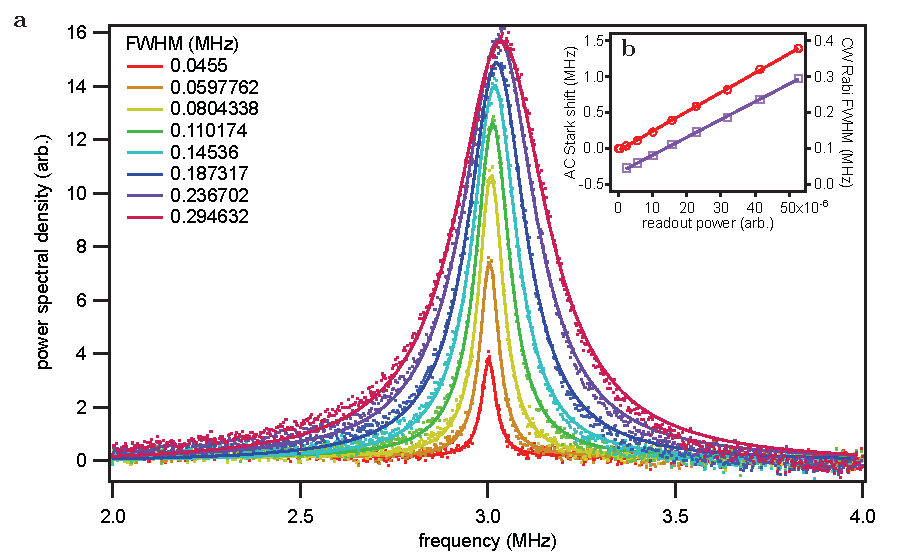
\includegraphics[width = 6in]{qfb_results_chapter/cw_rabi_and_gamma}
\end{center}
\caption[CW Rabi spectra and fits]{\textbf{a} CW Rabi spectra for a variety of measurement powers, from fairly weak measurement (red trace) to an optimal measurement power (magenta), and fits of the FWHM.  At the highest measurement power we observe a saturation in the height of the peak with increasing measurement strength.  This set of measurements was taken with a slightly odd paramp gain profile resulting in a sloping noise floor; this noise floor has been subtracted from the measured peaks for clarity and to improve the quality of the fits.  \textbf{b} AC stark shift (from Ramsey measurements, not shown; plotted in red, left axis) and the FWHM dephasing from \textbf{a} (plotted in purple, right axis), showing the linear relationship with measurement power.}
\label{fig:cw_rabi_and_gamma}
\end{figure*}

The purity of the qubit state in a single measurement can be revealed by averaging the ensemble in a different way.  Time-domain averaging for noisy oscillations will only work if the phase of the oscillations is essentially constant across every iteration of the experiment.  Instead, we can take the noisy experimental record from each individual experiment, convert it to a power spectrum using an FFT algorithm, and then average the power spectra together.  Korotkov calls this averaged power spectrum the \textit{CW Rabi spectrum}.  For high measurement efficiency and in the limit where the dephasing is dominated by the measurement, we should then clearly resolve a spectral peak corresponding to the measurement-dephased Rabi oscillations, centered at the Rabi frequency $\Omega_r$ and with a spectral width related to the total dephasing rate $\Gamma$ and a peak height above the noise floor related to the quantum efficiency $\eta$.  From reference \cite{korotkov_p2p}, the functional form of this peak is
\begin{equation}
S(\omega) = \frac{\Gamma \Omega_r^2 (\Delta V)^2}{(\omega^2 - \Omega_r^2)^2 + \Gamma^2 \omega^2}.
\end{equation}
The maximum occurs when $\omega = \Omega_r$ and has the value $S_{\rm max} = (\Delta V)^2 / \Gamma$.

Much of the most thorough CW Rabi spectrum data was taken in a cooldown prior to that corresponding to the published data set.  In this cooldown the measurement setup was not quite as well optimized as in the final data set, but the plots are illustrative so I will use them in this and the next section.  An example set of CW Rabi spectra are shown in Figure \ref{fig:cw_rabi_and_gamma}a.  For relatively weak measurement, the peak height is small.  As the measurement strength is increased, the peak height and width both grow due to the increased signal amplitude and measurement-induced dephasing rate.

Eventually, we reach an optimal measurement strength at which point increasing the magnitude of the signal does not increase the height of the peak.  This can be interpreted as an optimal trade-off between measurement accuracy and back-action.  Although the magnitude of the signal is increasing with increasing signal strength, the back-action of the measurement is broadening the peak such that even though the total power in the peak increases, the peak height remains fixed.  The slight rightward drift in the center frequency of the peaks is due to the power-dependent AC stark shift of the qubit which was not corrected for in this particular experiment.

\begin{figure*}
\begin{center}
	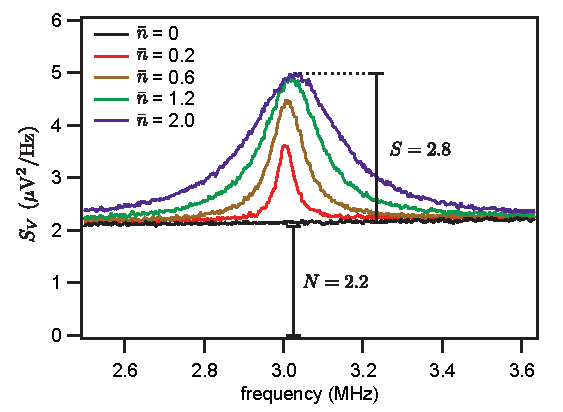
\includegraphics[width = 3.75in]{qfb_results_chapter/P2P}
\end{center}
\caption[Peak-to-pedestal ratio]{Measured CW Rabi spectra for several calibrated measurement powers, showing the saturation of the peak due to the measurement-disturbance tradeoff.  The ratio of the peak height to the noise floor provides a measurement of the total measurement efficiency $\eta$.}
\label{fig:P2P}
\end{figure*}

From \eqref{eq:bayesian_dephasing}, the spectral density of the noise floor of the CW Rabi spectrum for an ideal measurement is $S_0 = (\Delta V)^2 / 4 \Gamma_m$.  The ratio of the peak height to the noise floor (referred to as the \textit{peak-to-pedestal ratio} or \textit{P2P ratio} for short) is then calculated as $S_{\rm max} / S_0 = 4 \Gamma_m / \Gamma$.   From \eqref{eq:eta_basic_form}, we identify the ratio of dephasing rates as the quantum efficiency, allowing us to write $\rm P2P = 4 \eta$.  Thus, measuring the P2P ratio at the optimal measurement power described in the last paragraph provides another estimate of the total measurement efficiency $\eta$, complementing the Ramsey fringe technique discussed in section \ref{s:det_meas_eta}.  An example of this extraction is shown in Figure \ref{fig:P2P} with $\eta = S/4N = 0.32$ in this particular experiment.

\subsection{Quantum Zeno effect}

\begin{figure*}
\begin{center}
	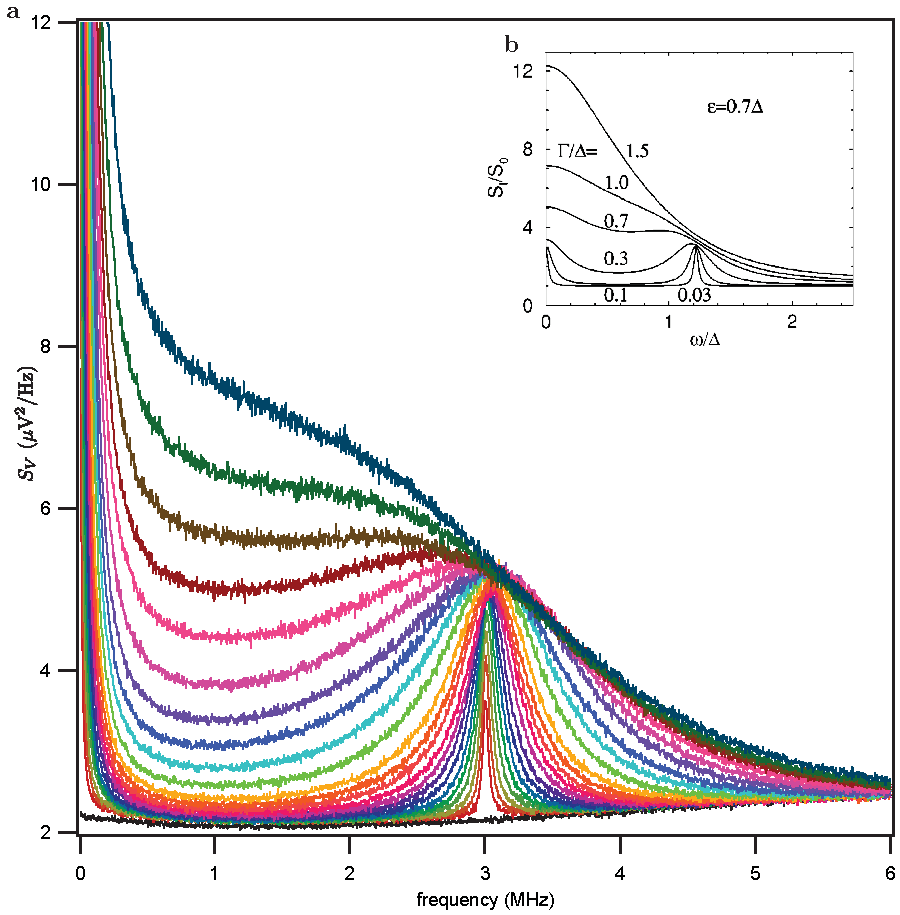
\includegraphics[width = 6in]{qfb_results_chapter/zeno}
\end{center}
\caption[CW Rabi spectrum and quantum Zeno effect]{\textbf{a} CW Rabi traces taken over a broad range of measurement strengths, smoothly covering the evolution from lightly-perturbed oscillations to telegraph-like measurement pinning of the qubit state.  \textbf{b} Theoretical curves for the same effect, showing beautiful qualitative agreement with the measured data.  Note that the parameter regime in this theory plot is not the same as that for the experimental data. In fact the parameters in the plot are described in the language for a quantum dot qubit read out with a quantum point contact, though the physics for the two systems is identical in the relevant regime.  Reproduced from reference \cite{korotkov_p2p}.}
\label{fig:zeno}
\end{figure*}

As seen in Figure \ref{fig:P2P}, the cavity photon number at which the measurement-disturbance tradeoff is saturated corresponds to a fairly small measurement power, whereas the power used for strong measurement is about 5 to 10 times larger.  What happens to the CW Rabi spectrum when the measurement is increased beyond the saturation point?  Qualitatively speaking, at some point the dephasing rate will exceed the Rabi frequency, and the qubit evolution will go from being something that looks like a noisy oscillation to something that looks mostly like random fluctuations with some weakly oscillating component.  There is no particular sharp transition which characterizes this changeover.

Measurements of the CW Rabi spectrum covering this entire regime are shown in Figure \ref{fig:zeno}.  At very strong measurement powers, the frequency of the peak begins to shift towards zero and becomes dramatically non-Lorentzian.  This transition from finite-frequency oscillations to a noisy spectrum centered at zero-frequency can be understood as an incarnation of the quantum Zeno effect.  Because the projective measurement time scale becomes short compared to the Rabi period, the strong measurement effectively pins the qubit state to one or the other eigenstate even though the dynamics of the system's free evolution should be oscillatory.

\subsection{Needles}

The aim of the feedback scheme is to stabilize the phase of the Rabi oscillations to that of some high-quality reference oscillator.  Or, equivalently, because phase fluctuations and small frequency fluctuations are interchangeable, we aim to stabilize the frequency of the Rabi oscillations to a precise value.  In the spectral domain, for a perfect reference oscillator, this type of oscillation corresponds to a $\delta$-function in frequency (any real oscillator will of course have a finite spectral width).  Thus, the signature of effective feedback control of the qubit is the appearance of a sharp, narrow peak on top of the CW Rabi spectrum.  Because the linewidth of the classical oscillator is sub-hertz and out experiments last for at most a millisecond or so, our FFT point spacing will always be larger than the width of this peak, implying that the signal in the experiment is literally one elevated point in the FFT.  Because of the extreme narrowness, we often refer to this peak as a \textit{needle}.

\begin{figure*}
\begin{center}
	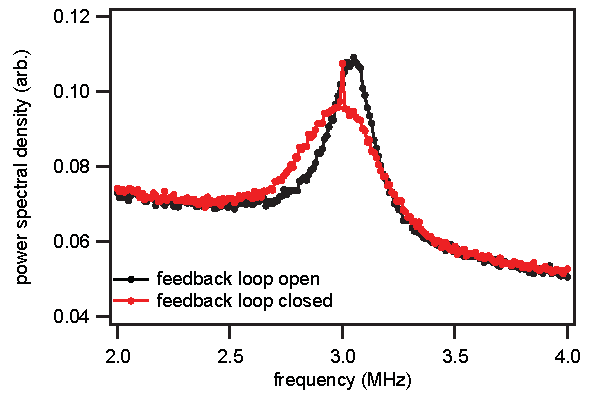
\includegraphics[width = 4in]{qfb_results_chapter/first_fb}
\end{center}
\caption[First observation of feedback stabilization]{The first confirmed feedback needle.}
\label{fig:first_fb}
\end{figure*}

Successful feedback was first measured on September 24, 2011, at about 5:30pm.  It was quite an exciting moment, not least of all because it was extremely unclear if we had really seen an effect at first.  The needle was barely visible above the top of the CW Rabi peak, and worse, because it is always exactly one point wide, it was difficult to determine if we were seeing a signal or just a small fluctuation in the noise.  After a bit of tuning of the feedback parameters, we were able to bring the needle conclusively above the peak.  The data taken at this moment are shown in Figure \ref{fig:first_fb}.  Cheers went up, ``quantum feedback!''

\begin{figure*}
\begin{center}
	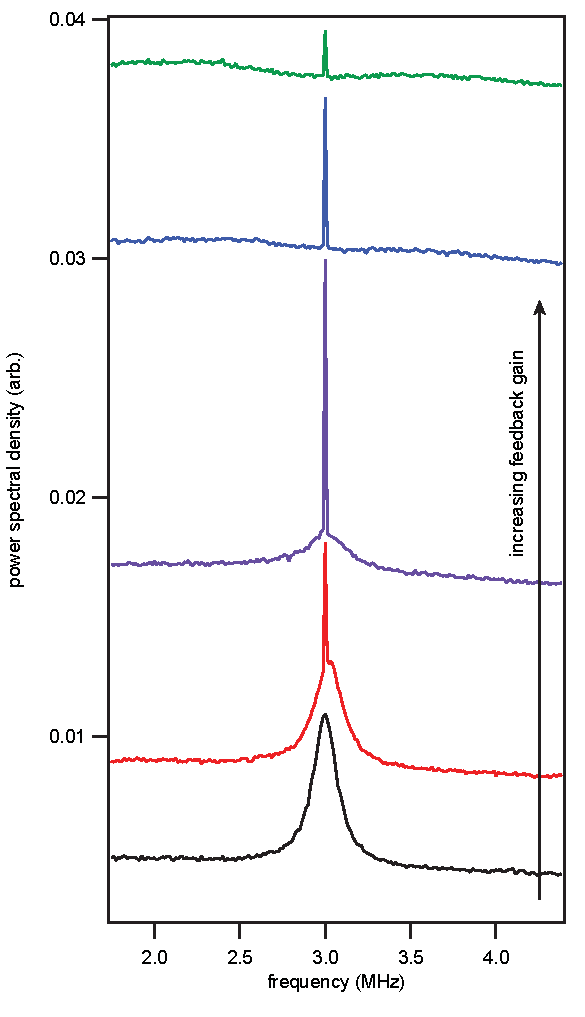
\includegraphics[width = 4in]{qfb_results_chapter/needle_zoo}
\end{center}
\caption[CW Rabi spectrum and needles versus feedback strength]{An assortment of CW Rabi spectra with feedback needles.  Each trace is taken with the same measurement power, with feedback strength increasing for each trace moving vertically up the plot, starting with no feedback in black.  Traces are offset for clarity.}
\label{fig:needle_zoo}
\end{figure*}

Because the needle has essentially zero spectral width while the CW Rabi spectrum itself is continuous, the needle can be more clearly observed by reducing the FFT point spacing, reducing the absolute power spectral density for every point except the needle.  A set of spectra with feedback from the final published data set are shown in Figure \ref{fig:needle_zoo}.  The black trace is taken with the feedback loop open.  The red trace shows a low feedback gain, where most of the oscillation power remains unsynchronized.  The purple trace represents the optimum feedback strength for this measurement power, with about half of the total Rabi peak power contained in the needle.  The blue and green traces show feedback gains which are above the optimum, where the feedback correction applied to the system is larger than the correction needed to undo the effect of the measurement dephasing.  In this regime, characteristic ``wings'' in the spectrum appear, particularly visible in the green trace.  This can be intuitively understood as the feedback ``oversteering'' the qubit oscillation frequency; the actual correction needed to stabilize the qubit is a relatively small frequency shift, but because the gain is large, the frequency correction becomes large, developing two peaks at a detuning proportional to the feedback gain.

\section{Time-domain measurements}

The needles alone are conclusive evidence of successful quantum feedback, and provide a complete quantitative picture of the feedback quality.  However, they do not impressively demonstrate the result because Rabi oscillations are not usually analyzed in the frequency domain.  Time domain measurements of the stabilized state viscerally demonstrate the feat accomplished in this experiment, because the time-domain equivalent of a needle is a \textit{coherent oscillation that does not decay}.  As long as the phase of the reference oscillator is stable with respect to the rest of the experiment, time-domain averaging is possible.

\begin{figure*}
\begin{center}
	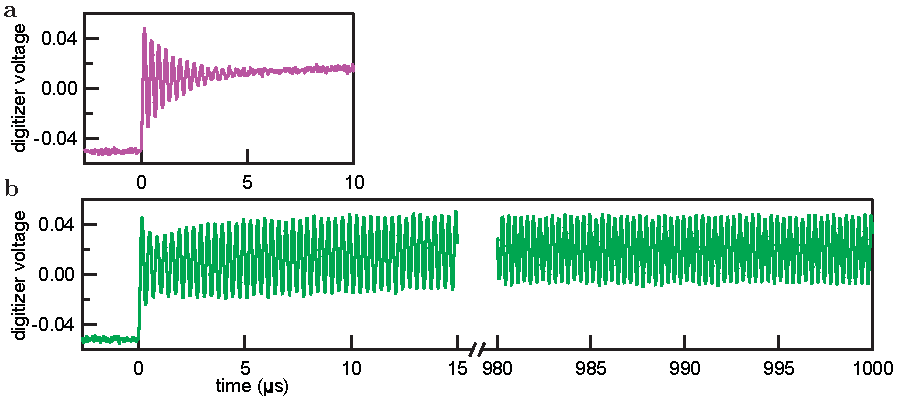
\includegraphics[width = 6in]{qfb_results_chapter/time_domain}
\end{center}
\caption[Stabilized time-domain Rabi oscillations]{\textbf{a} A typical averaged time-domain Rabi oscillation, showing the characteristic exponential decay associated with dephasing. \textbf{b}  Feedback-stabilized time domain Rabi oscillations.  Adapted from reference \cite{vijay_stabilizing_2012}.}
\label{fig:time_domain}
\end{figure*}

Time-domain-averaged Rabi oscillations are shown in Figure \ref{fig:time_domain}.  A weak measurement is constantly on, while the Rabi drive turns on at $t = 0$.  Figure \ref{fig:time_domain}a shows the typical exponentially-decaying oscillations for a qubit with a finite decoherence rate.  In this case, the dephasing is dominated by the measurement, so the oscillations decay relatively quickly.  Without a measurement, the oscillations decay on a timescale of about 10 $\mu$s.  In Figure \ref{fig:time_domain}b, the feedback loop is closed when the Rabi drive turns on.  The oscillations show an initial transient period while the qubit phase evolves to match that of the reference oscillator, and then stabilize to a finite contrast which does not decay in time.  The feedback efficiency is related to the contrast of the stabilized oscillations compared to the full-scale oscillations; the contrast here is about 50\%.  Here two measurements are stitched together, showing an initial 15 $\mu$s of stabilized oscillation, and another 20 $\mu$s after leaving the feedback loop closed for about 1 ms.  In this data, no post-selection has been done to remove the effect of thermal excitations out of the $ \{ \ket{0},\ket{1}\}$ manifold, which is visible as a slight upwards drift after the Rabi drive turns on.

\begin{figure*}
\begin{center}
	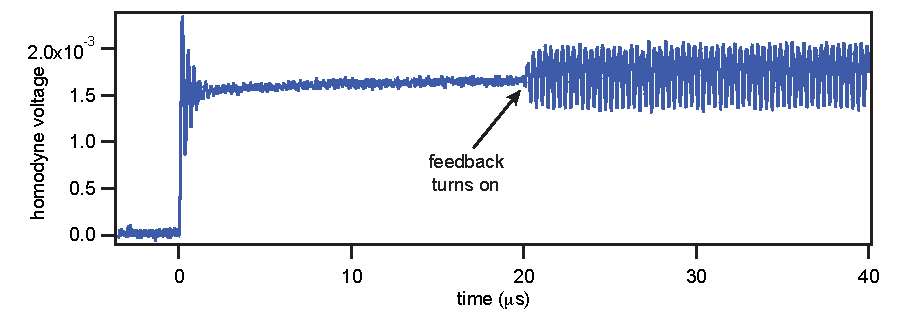
\includegraphics[width = 6in]{qfb_results_chapter/rephase}
\end{center}
\caption[Feedback re-phases a mixed state]{Time domain Rabi trace, showing the effect of delayed activation of the feedback control.  The  contrast is reduced compared to Figure \ref{fig:time_domain}b because this data was taken on a prior cooldown under different, less-optimized parameters.}
\label{fig:rephase}
\end{figure*}

Because the weak measurement extracts information about the phase of the qubit, the feedback stabilization will work regardless of the initial phase of the qubit oscillations.  Furthermore, because the feedback locking mechanism occurs in each individual iteration of the experiment, the feedback loop will still lock the oscillation phase even if the qubit's phase is completely randomized.  In other words, if we start with an ensemble of qubits in a completely mixed state, and then turn the feedback on, the ensemble will be re-cohered into a pure state (with a purity set by the feedback efficiency).  This effect is shown in Figure \ref{fig:rephase}, where we have delayed closing the feedback loop until 20 $\mu$s after the Rabi drive is turned on.

\section{Tomographic validation}

\begin{figure*}
\begin{center}
	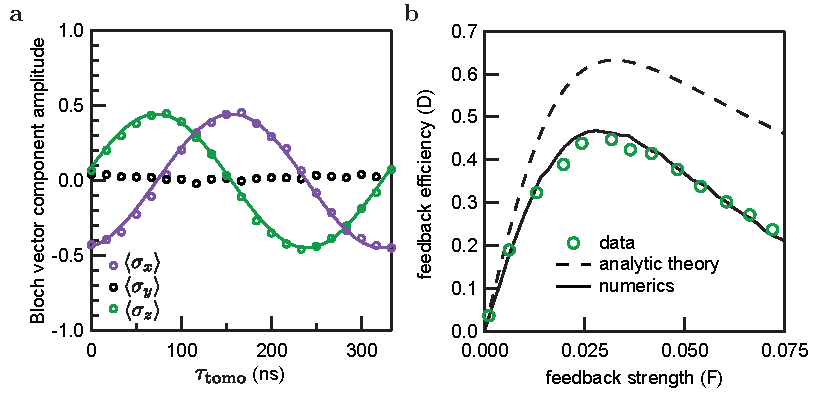
\includegraphics[width = 5.5in]{qfb_results_chapter/fb_tomo}
\end{center}
\caption[Tomographic validation of feedback]{\textbf{a} Tomographic validation of the feedback-stabilized qubit state, showing the measured Bloch vector components as a function of $\tau_\mathrm{tomo}$.  The Bloch vector components $\xpec{\sigma_x}$ and $\xpec{\sigma_z}$ are, as expected, sinusoidal oscillations with a $\pi/2$ phase shift, and an amplitude of 0.45, corresponding to a feedback efficiency $D = 0.45$.  The $\xpec{\sigma_y}$ component is essentially zero, as expected for driven Rabi oscillations in the $x-z$ plane.  \textbf{b} Tomographically-measured feedback efficiency $D$  versus feedback strength $F$.  The dashed line corresponds to the simple analytical theory, while the solid black line is based on numerical analysis including the effect of finite loop delay.  Adapted from reference \cite{vijay_stabilizing_2012}.}
\label{fig:fb_tomo}
\end{figure*}

In order to validate the quantum nature of the stabilized qubit state and precisely assess its purity, we stop the feedback after a time $(80 \ \mu\mathrm{s}) + \tau_\mathrm{tomo}$ and perform a complete tomographic reconstruction of the state of the qubit.  By repeating this experiment with a range of $\tau_\mathrm{tomo}$ covering one fully stabilized oscillation, we can fit the resulting reconstruction of the Bloch vector components to sinusoids and extract the feedback efficiency $D$ as the length of the Bloch vector.  By repeating this experiment for a variety of feedback and measurement strengths, we can find the best global performance of the feedback.  Tomographic reconstruction of a feedback-stabilized oscillation is shown in Figure \ref{fig:fb_tomo}a for the experimentally-determined optimal conditions $\bar{n} = 0.47$ (corresponding to a measurement-induced dephasing rate $\Gamma_\varphi/2\pi = 134$ kHz) and $F = 0.032$.  The reconstructed state is a coherent oscillation in the $x-z$ plane at the Rabi frequency with a Bloch vector length of 0.45, corresponding to $D = 0.45$.

In order to compare these results to the theoretical prediction for the feedback efficiency, we examine the dependence of the efficiency on the feedback gain $F$, shown in Figure \ref{fig:fb_tomo}b.  The efficiency quickly rises as the feedback strength is turned up, peaks, and then more gently slopes back down as the feedback correction being applied to the system becomes too large.  Plotted along with the data are the predictions for the simple analytic result
    \begin{equation}
    D=2 \left(\displaystyle \frac{1}{\eta}\, \frac{F}{\Gamma/\Omega_0}
+\frac{\Gamma/\Omega_0}{F} \right)^{-1}
    \end{equation}
as well as the results of a complete numerical calculation which includes the effect of the finite loop delay, using the measured efficiency $\eta = 0.4$ and the total dephasing rate $\Gamma/2 \pi = 154$ kHz.  Details on the numerical calculation can be found in the supplementary information of reference \cite{vijay_stabilizing_2012}.





















